\section{Introduction to Prefix search}
The indices created so far only return the list of article titles where there is an exact match of the query. This can inhibit the user experience as this search form might miss relevant articles where a buzzword simply is written in another tense or in  pluralism, which could add different suffixes to the word. To improve the user experience of the search engine and to explore the data structure of tries, indices that support prefix search were implemented.

Prefix search enables users to input partial words and retrieve relevant results that match the given prefix. If the user want to search for a prefix they simply need to add a star as a suffix of their query. For instance, when typing "pre*" in a search engine, the indices will return the title of all articles where a word with the prefix "pre" is present. 

\section{Tries}
To implement prefix search efficiently, one effective data structure that can be employed is a trie, also known as a prefix tree. A trie is a tree-like structure that stores a database, with each edge, or node depending on the implementation, representing a character in the string. Tries offer an efficient approach for prefix search by allowing rapid traversal and retrieval
%\footnote{The name of the data structure "trie" comes from the middle syllable of "retrieval"}
of words based on their prefixes.

\begin{figure}[b!]
    \centering
    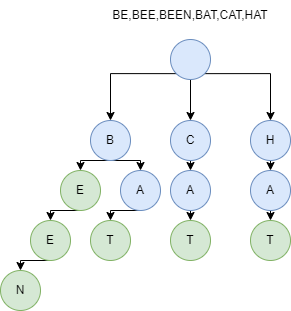
\includegraphics[width=.5\textwidth]{LaTeX/Figures/Tries/trie.png}
    \caption{Example of a trie for the database BE, BEE, BEEN, BAT, CAT, HAT. Green nodes are accepting nodes. }
    \label{fig:trie-st-example}
\end{figure}

Formally, a trie is a rooted tree where each edge, or child, has a distinct label. Each key in the database corresponds to a path from the root to an accepting node, for which the key is denoted its "associated key". Most typically, the keys in a trie are strings and each label is an individual character. However, it is possible to use tries for other alphabets, e.g. containing numbers, or entirely other content where only the concept of a "prefix" is required. This section focuses on strings and with characters as the edge labels. Extensions such as the compact trie (see section \ref{sec:compact_tries}) may use substrings. 

When a key is looked up in a trie, a depth-first-search is used to traverse the prefix tree, matching each character in the key with edges along the way, until an "accepting node" is found. These nodes can contain satellite data such as a pointer to an array, and they are marked as accepting nodes. Typically, a child containing a special character not in the alphabet such as "\$" is added to indicate that the parent is an accepting node, but in this section simply the presence of satellite data marks the node. Notably, the nodes themselves do not store their entire associated key, but rather the key is induced by the node's position relative to the root. 

Figure \ref{fig:trie-st-example} shows an example of a trie for the database "BE, BEE, BEEN, BAT, CAT, HAT". Each node can have satellite data indicating that the word consisting of the characters from the root to the node exists in the database. These are marked as green on the figure. 

\subsection{Constructing a trie} \label{sec:Constructiontire}

When constructing a trie, words in the database are read one-by-one and inserted into the trie. This is done by performing the following steps:

\begin{enumerate}
  \item For each word in the database iterate through the characters of the word.
  \item Begin at the root node and check if there is a child node representing the current character of the word. 
  \item If an edge corresponding to the current character exists, move to that child node and continue to the next character of the word.
  \item If a child node does not exist for the current character, add the character to the children of the current node. Move to the newly created node.
  \item Do step 3 and 4 for all characters in the word until the end is reached. 
  \item Mark the last node as an accepting node since its associated key is in the database and optionally add satellite data to the node. 
\end{enumerate}

\subsection{Possible structures of tries} \label{sec:posStrucOfTrie}

There are several ways of designing a trie and choosing how to traverse it and how to store the children. The best method depends on the size of the alphabet $|\Sigma|$, the expected length and amount of words, and so on. 

One way is to maintain the children of a node as pointers in an array of size $|\Sigma|$. When looking up a character in the key, the child corresponding to that character can then be found in constant time by indexing into the array, see figure \ref{fig:trie_array}. This has the advantage that it takes $O(s)$ time to locate the node of a key, where $s$ is the number of characters in the key. This is comparable to a hash table, where a hash function typically also uses $O(s)$ time to hash a string before returning its value in the table. A disadvantage of this array approach is that it requires each node to store an array of length $\Sigma$ where most of the spaces would be empty. In total this uses $\Theta(p\cdot\Sigma)$ space, where $p$ is the size of the trie, which is equal to the total number of possible prefixes of all words in the input. 

\begin{figure}[ht!]
    \centering
    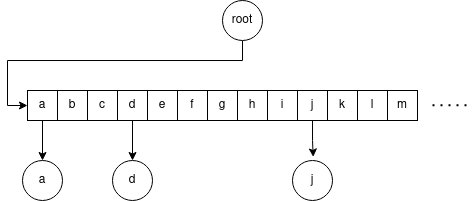
\includegraphics[width=.9\textwidth]{LaTeX/Figures/Tries/Trie_array.png}
    \caption{A version of a trie where nodes maintain an array of each character in the alphabet to quickly find the child matching a given character. }
    \label{fig:trie_array}
\end{figure}

Another way that uses less space is to maintain the children of a node as a linked list, with each link containing the character on the node/edge and a pointer to that child node. The space used is upper bounded by the size of the alphabet but no longer lower bounded by it, resulting in $O(|\Sigma|)$ space for each node in the worst case and on average better. However, now the time for locating the child matching a character is proportional to the number of children, which is also $O(\Sigma)$. 

As mentioned above, looking up a key in a trie where it takes constant time to find the child of a node matching a character is similar to a hash table, if the hash function uses $O(s)$ time for a string of length $s$. Conversely, a hash table can also be used internally in a trie to locate the children of a node if the alphabet is expected to be large but each node is expected to have few children. This approach uses $O(p\cdot\Sigma)$ space for the trie in total but because of the constant lookup time for each character, uses $O(s)$ time to locate a key. This approach becomes less efficient if the time to calculate the hash value of a string is not proportional to the length of the hashed string, as section \ref{sec:index9.1} regarding Index9.1 will discuss. 


\subsection{Constant vs non-constant alphabets}

A few factors in the complexities of the tries change when the alphabet is no longer constant or known from the beginning. The method of using a constant size array of pointers is not usable in this scenario and the linked list gets a worse complexity. However, an interesting thing about the linked list solution here is that when the values are inserted in order of first appearance in the input, the most common letters are among the first characters, and less common characters (like chinese and greek letters in the Wiki files that are in English) are further in the list. In practice, this means that when searching for an English word, the key to the next edge, if it exists, is expected to be found within the first part of the linked list, compared to some of the input files in which the alphabet has a size of $|\Sigma|\geq2000$ characters. 



\subsection{Compact tries}\label{sec:compact_tries}
A compact trie is a more memory-efficient trie. In a compact trie, common prefixes among different keys are shared, resulting in space savings compared to a regular trie. This compression technique is achieved by combining consecutive nodes in the trie that have only a single child into a single node. By eliminating redundant nodes, compact tries can significantly reduce memory usage, making them more space-efficient than regular tries. When using the version of a trie where nodes associated with a key has a child containing a $\$$ sign, a compact trie guarantees that every non-$\$$ node has at least two children. This then implies that the total number of nodes in the compact trie is proportional to the number of words inserted into it. 

In general, uncompressed tries have faster insertion and deletion operations compared to compact tries. This is because compact tries require additional operations to compress and decompress nodes when modifying the tree structure. On the other hand, regular tries can directly add or remove nodes without the need for compression.

Searching a regular tire would also be slightly faster, as its operations do not involve any string matching operations.
 
%Applications like the Aho-Corasick algorithm

\subsection{Suffix trees}\label{sec:suffixtree}
A suffix tree is a data structure that efficiently represents all the suffixes of a given string. It provides a compact representation of the text that allows for efficient searching and pattern-matching operations. A suffix tree is constructed by organising the suffixes of a string into a trie structure.

Tries and suffix trees share some similarities in terms of their underlying principles and applications. Both tries and suffix trees utilise the concept of prefixes. In a trie, each node represents a prefix of a string, and the edges represent characters that extend the prefix. Similarly, in a suffix tree, each node represents a substring or a prefix of a suffix, and the edges correspond to the characters that extend the substring. The path from the root of the tree to a leaf node represents a complete suffix of the original string.

The space complexity of a suffix tree is $O(n)$ as the size of the tree is directly proportional to the length of the input text - for every suffix it is possible to pick the position where the suffix starts. Like in the prefix search tries, accepting nodes can store article lists as a representation of where the suffix is present. 

The construction of a suffix tree can easily be done in a naive and inefficient way, by simply adding all suffixes of a text to a trie. Efficient construction of a suffix tree is much trickier. A more practical construction can be achieved using various algorithms, such as Ukkonen's algorithm or McCreight's algorithm. These algorithms efficiently build the tree in linear time, making suffix trees a practical choice for processing large search text.

Suffix trees enable fast pattern matching by providing an efficient way to search for substrings or patterns within the text. By traversing the tree, patterns can be found in linear time to the length of the pattern being searched. This is relevant when solving string matching problems, like in the section Full Text searching. 
